For at danne overblik over software-udviklingen inden det egentlige design, laves bruges N+1 modellen\footnote{\url{http://goo.gl/kU89oe} [2014-11-02]}.
Denne beskriver fire faser som tager hånd om de overordnede ting inden for software, alt sammen med use-cases som den røde tråd.
De fire faser er:

\begin{enumerate}
	\item Logical View
	\item Deployment View
	\item Implementation View
	\item Data View
\end{enumerate}

Ud over disse punkter tænkes der også en overordnet fejl-håndtering ind i projektet. Disse punkter er beskrevet i detaljer herefter.

\subsection{Logical View (JC)}
%% SW arkitektur: Logical View

Logical View skal danne et overblik over hvilke softwarepakker der befinder sig på platforme. Blokkene inde i de respektive pakker kan sammen med domænemodellen, hjælpe med at give et overblik over hvilke klasser og kernemoduler der skal bruges.

\begin{figure}[htbp] \centering
{\includegraphics[scale=0.7]{filer/systemarkitektur/logical_view_devkit}}
\caption{Logical view for Devkit8000 illustrerer hvilke softwarepakker der befinder sig på Masteren }
\label{fig:Logical View Devkit8000}
\end{figure}

Figur \ref{fig:Logical View Devkit8000} illustrerer hvilke softwarepakker der ligger på Masteren. I bunden er \textit{Device drivers}-pakken som håndterer SPI kommunikationen imellem Master og Enhed. I midten ligger \textit{Hardware API}-pakken som håndterer protokol-vedtægter ifm. kommunikationen. \textit{Application}-pakken tager sig af alt UI samt log og fejlhåndtering.

\clearpage

\newenvironment{figure1}[1][]{\begin{figure}[#1]\vspace{3.0cm}}{\vspace{1.0cm}\end{figure}}
\begin{figure1}[htbp] \centering
{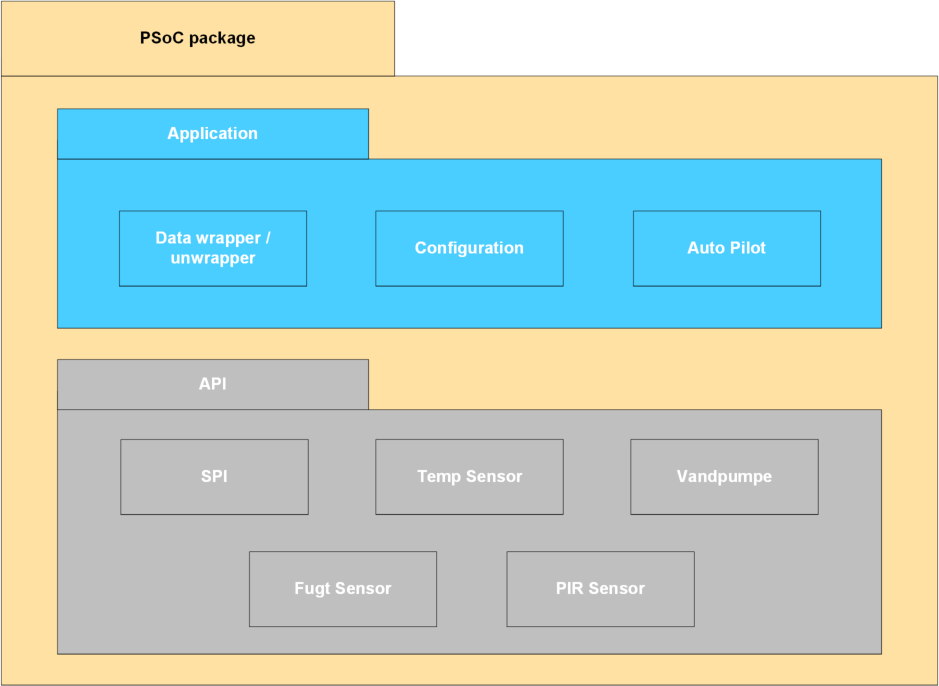
\includegraphics[scale=0.7]{filer/systemarkitektur/logical_view_psoc}}
\caption{Logical view for PSoC illustrer hvilke software pakker der befinder sig på enhederne}
\label{fig:Logical View PSoC}
\end{figure1}

Figur \ref{fig:Logical View PSoC} illustrerer hvilke softwarepakker der ligger på Enhederne. \textit{API}-pakken består af den software som håndterer hardwaren, dvs. den tager imod input og får formateret det til noget brugbart for \textit{Application}-pakken. \textit{Application}-pakken håndterer den indsamlede data som den får fra sensorene igennem \textit{API}-pakken. Denne data sammensættes iht. protokollen og sendes til API pakken som får det sendt til Devkit8000. Pakken skal også håndterer data fra Devkit8000 til at konfigurerer de parametre der styrer automatiseringen af vandingen.



\clearpage
\subsection{Deployment View (JC)}
%% SW arkitektur: Deployment View

Deployment view skal illustrere hvor hvilke lag af software ligger på vores platforme. Devkit8000 kører linux og har derfor flere software lag end PSoC'en.
 
\vspace{15 mm}

\begin{figure}[htbp] \centering
{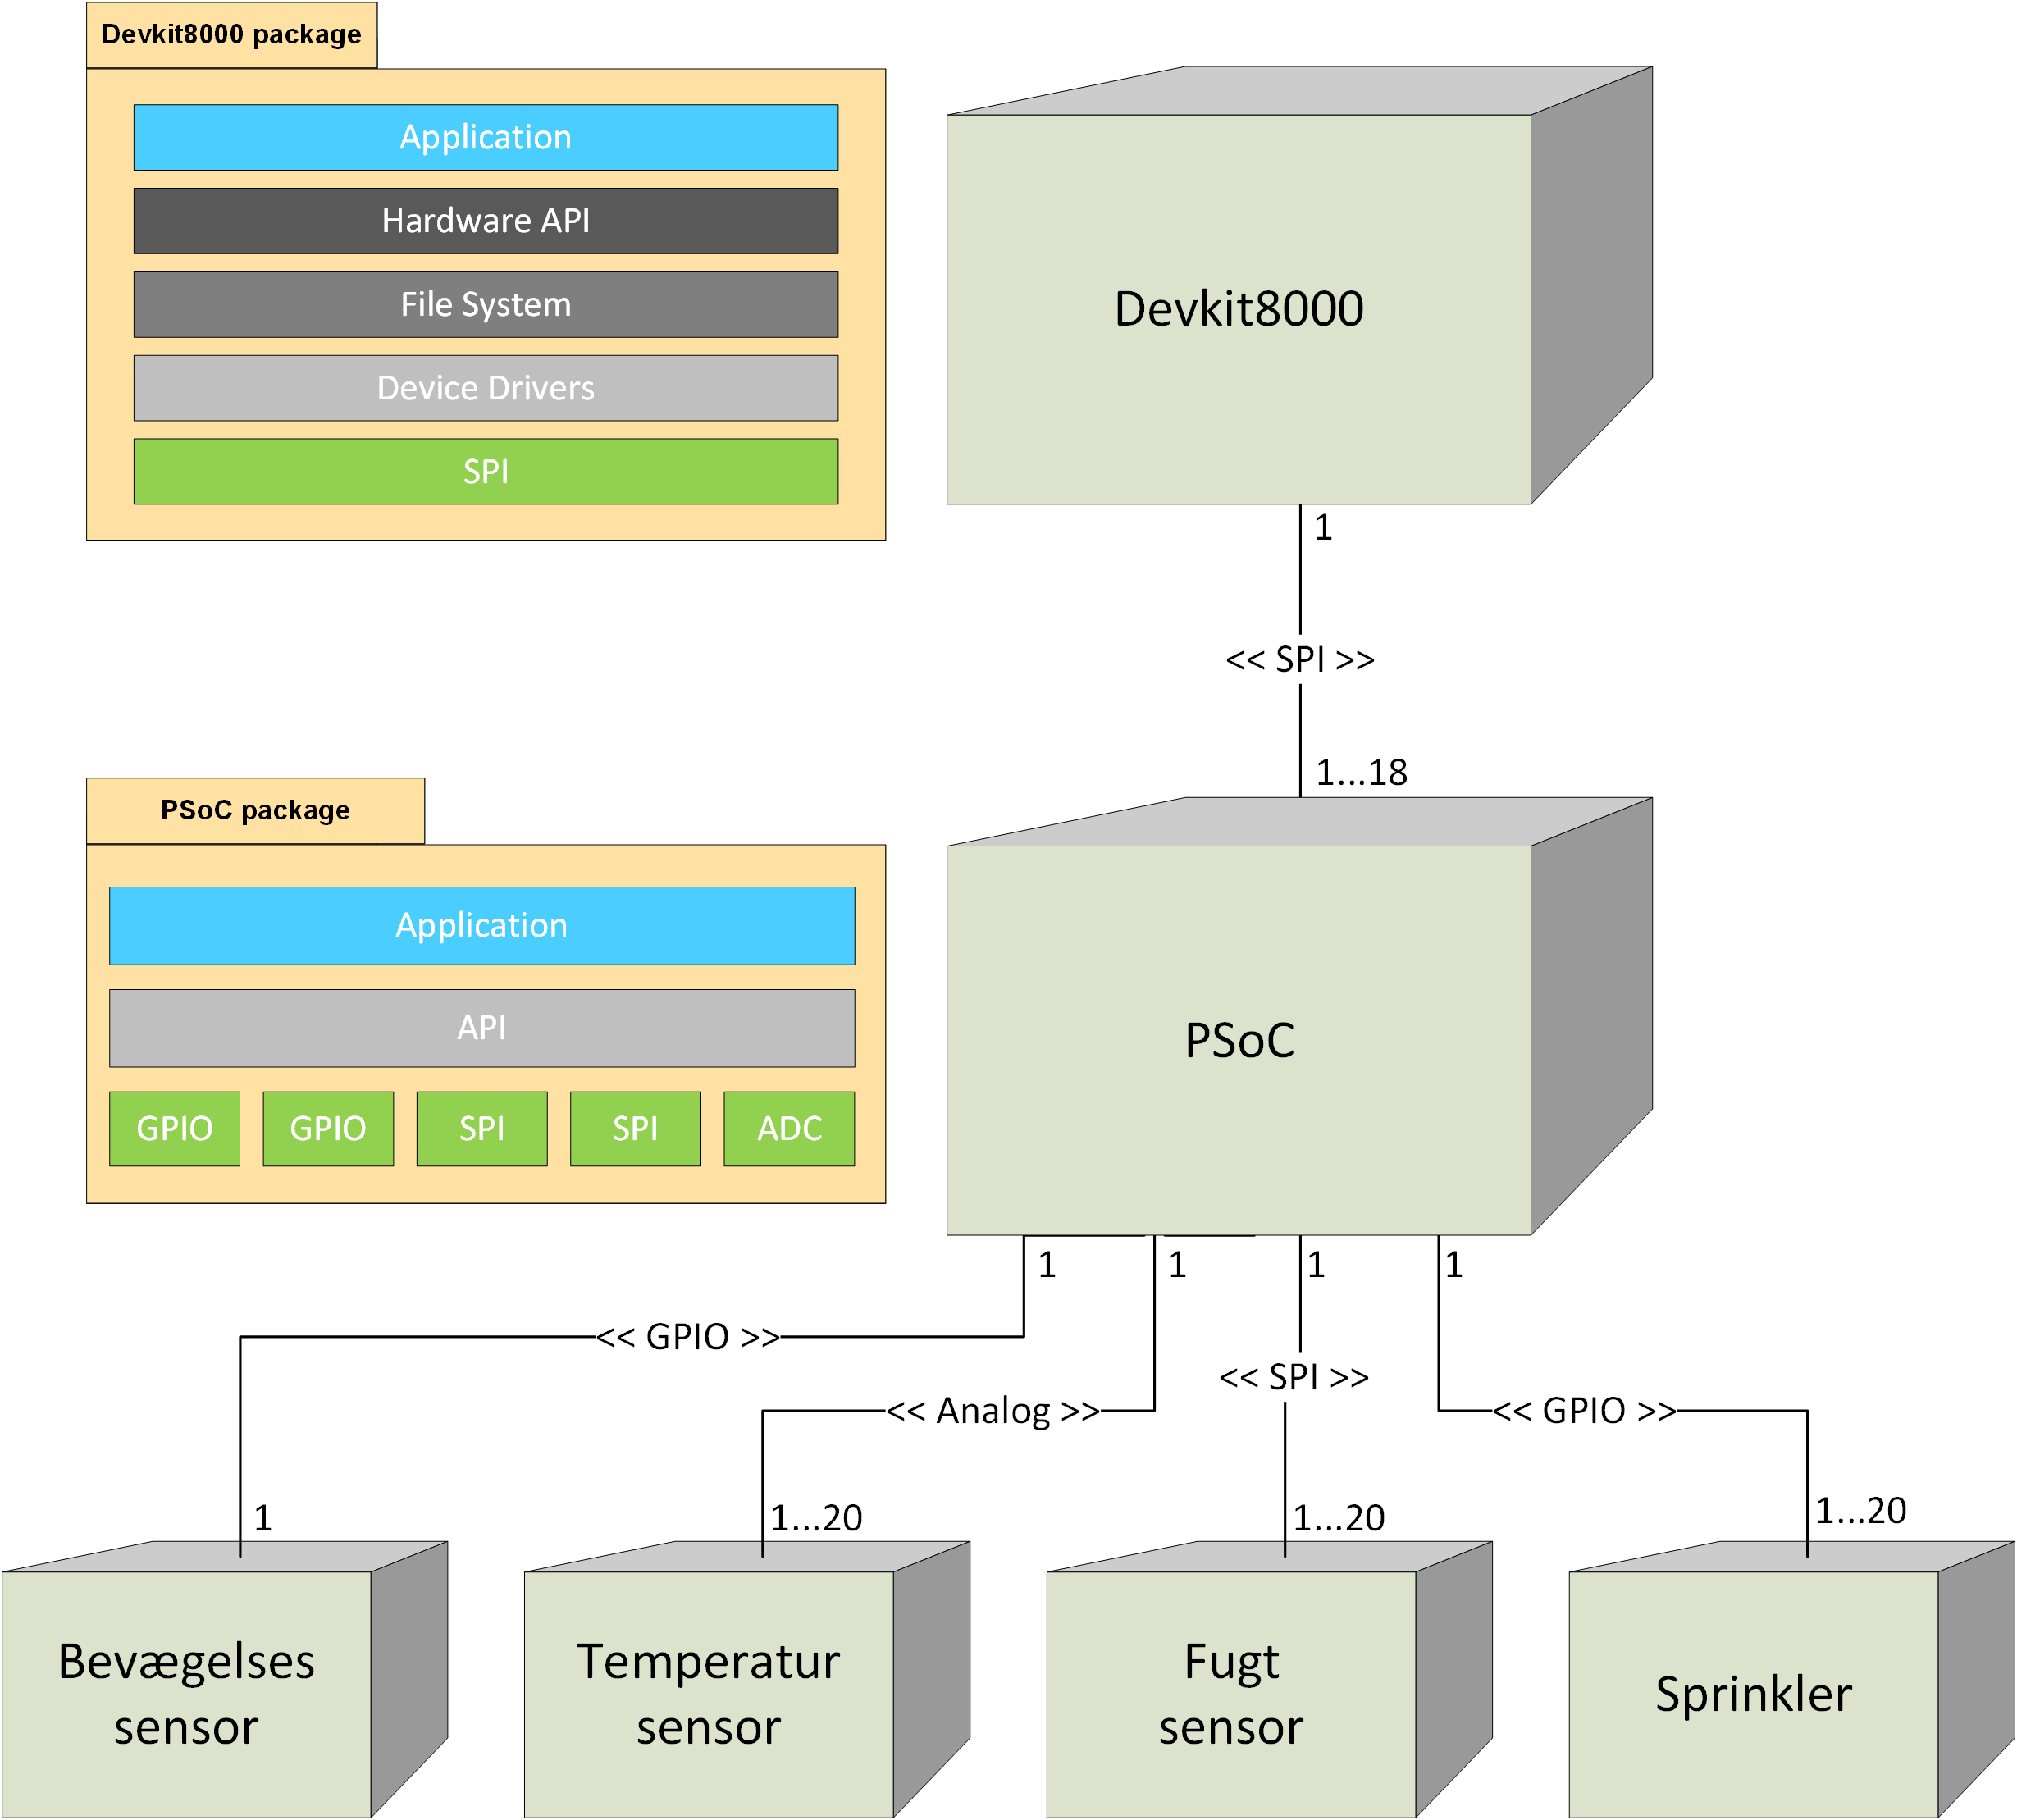
\includegraphics[scale=0.7]{filer/systemarkitektur/Deployment_model}}
\caption{Deployment model illustrere de forskellige software og hardware(grønne) lag}
\label{fig:Deployment Model}
\end{figure}

\vspace{5 mm}

\subsubsection{Devkit8000}
\textit{Applications} laget består af alt den software som har med brugeren at gøre, dvs. UI og tilhørende controllers. Applicationslaget tager imod input fra brugeren og reagere på det enten ved at kalde nogle af sine egne controllers eller sende kommandoer til hardware APIen. Laget skal desuden få data fra nedenstående lag til at fremstå overskueligt over for brugeren.

\clearpage

\textit{Hardware API} laget består af almindelige klasser som gør brug af file systemets kommandoer som f.eks open og close.

\textit{File System}

\textit{Device Driver} laget består af den software som håndtere alt hardware input og output. Hardware proxys inklusiv.

\textit{HW connection (grønne bokse)} laget viser hvilke hardware in/out der er til devkittet

\subsubsection{PSoC}

\textit{Applications} laget håndtere den indsamlede data som den får fra sensorene igennem API'en. Denne data sammensættes ifølge protokollen og sendes til API'en som får det sendt til devkittet. Laget skal også håndtere data fra devkittet til at konfigurere de parametre der styre automatiseringen af vandingen som applications laget også håndtere.

\textit{API} laget består af den software som håndtere hardwaren. dvs den tager imod input og får formateret det til noget læseligt til applications laget. Derudover står den for at få sendt de informationer applicationslaget ber om på en effektiv og sikker måde.

\textit{HW connection (grønne bokse)} laget viser hvilke hardware in/out der er til PSoC'en


\subsection{Implementation View (BS)}
%% SW arkitektur: Implementation View

Inden programmerne designes, fastlægges en struktur for kildekoden. På den måde er det nemmere for flere programmører at arbejde med delene i programmet samtidigt.

Strukturen skal være som vist i figur \ref{fig:implementationview}. Under mappen ''Kildekode'' skal hver klasse have en mappe med dertil hørende filer. Ligeledes med ''Testprogrammer'' mappen, som indholder testprogrammer som verificerer funktionaliteten af de enkelte moduler.
Mappen ''Kompilerede programmer'' er til de endelige programmer.

\begin{figure}[htbp] \centering
{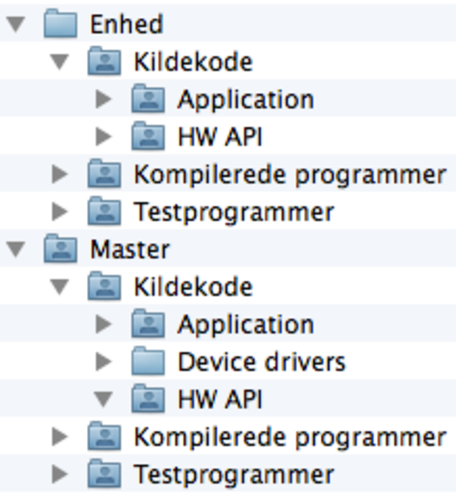
\includegraphics[scale=0.7]{filer/pics/SW-Implementation-View}}
\caption{Mappestruktur for software-kilder}
\label{fig:implementationview}
\end{figure}

\subsection{Data View (BS)}
%% SW arkitektur: Data View

I forbindelse med EasyWater8000s log skal der gemmes data på en nem og håndterbar måde. Det skal være muligt at gemme følgende data:

\begin{enumerate}
	\item Tidsstempel
	\item Temperatur
	\item Fugtighed
	\item Bevægelse
	\item Vanding
\end{enumerate}

Ydermere skal disse informationer gemmes for hver Enhed. Så hvis der er 18 huller med i alt 18 Enheder, skal ovenstående gemmes for alle 18 enheder.

Når informationen skal præsenteres for brugeren skal det ske i en tabel som vist på figur \ref{fig:GUI-log-alle} i afsnit \ref{subsec:GUI}, data for en enkelt enhed som på figur \ref{fig:GUI-log-enhed} i afsnit \ref{subsec:GUI} eller på en graf så man kan se ændringer over tid som vist på figur \ref{fig:log-graf}.

\begin{figure}[htbp] \centering
{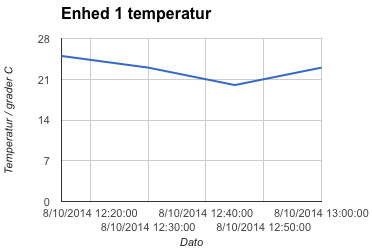
\includegraphics[scale=0.5]{filer/pics/SW-Log-graf}}
\caption{Graf for temperatur for én Enhed}
\label{fig:log-graf}
\end{figure}

Tabellen skal have en fane for hver opkoblet Enhed. Her kan man se informationer fra hver enkelt Enhed. Det bør også være muligt at se alle enheders informationer samtidigt.

Dataen struktureres i semikolon-separerede filer (\verb+.csv+) på Master. Hver Enhed har en fil hvor alle data er samlet med udgangspunkt i strukturen vist i liste \ref{list:log-csv-struktur}.

\begin{lstlisting}[caption=Semikolon-separeret datafil til log af enheder, label={list:log-csv-struktur}]
<enheds-nr>;
<KP-nr>; <dato>; <temperatur>; <fugtighed>; <bevaeglse>; <vanding>;
<KP-nr>; <dato>; <temperatur>; <fugtighed>; <bevaeglse>; <vanding>;
...
<KP-nr>; <dato>; <temperatur>; <fugtighed>; <bevaeglse>; <vanding>;
\end{lstlisting}

Dette resulterer i en filstruktur som vist på liste \ref{list:log-fil-struktur} hvis der er koblet 18 Enheder op på Master.

\begin{lstlisting}[caption=Filstruktur for logfiler på Master, label={list:log-fil-struktur}]
<log>/
  <enheds-nr1>.csv
  <enheds-nr2>.csv
  ...
  <enheds-nr17>.csv
  <enheds-nr18>.csv
\end{lstlisting}

Hyppigheden for målingerne og logningen er beskrevet i de ikke-funktionelle krav, \ref{header:ikke-funk}.


\subsection{Fejl-håndtering (JC)}
%% SW arkitektur: Fejlhåndtering

Systemet kan håndterer fejl og disse vil blive gemt i en fejllog som bliver gemt på Master. 

Fejlhåndteringen bliver klaret af en klasse på Devkit8000 som håndterer at skrive det rigtige fejl ud i en \verb+.txt+-fil. Klassen vil blive kaldt med en fejlkode hver gang fejl opstår. Klassen forstår så at skrive den rigtige fejl ind i txt filen ud fra den pågældende fejlkode den har modtaget som attribut. 

Alle funktioner vil returnere et negativt heltal som repræsenterer en fejlkoden som klassen kan tolke på.

\begin{figure}[htbp] \centering
{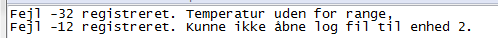
\includegraphics[scale=0.7]{filer/pics/Errortxt}}
\caption{udsnit af Error log}
\label{fig:ErrorLog}
\end{figure}

Billedet på figur \ref{fig:ErrorLog} viser hvordan 2 fejl i error-loggen kunne se ud.

\subsection{Kommunikationsprotokol (BS+MK)}
%% SW arkitektur: Kommunikationsprotokol

En del data skal flyttes mellem Master og de tilkoblede Enheder. Her følger beskrivelsen af hvordan data pakkes mellem de to dele. Den elektriske protokol som anvendes er SPI.

Opsætningen er som følger:
\textit{Hastighed
SPI mode
Antal bits}

Ud fra UC-beskrivelserne er der identificeret følgende scenarier hvor der sendes data mellem Master og Enhed.

\begin{enumerate}
	\item Master kontrollerer om Enhed er koblet til systemet (UC1)
	\item Master sender parametre til Enhed (UC2)
	\item Enhed aktiveres eller deaktiveres af Master (UC3)
	\item Master beder om data fra Enhed (UC4)
	\item Enhed sender data til Master (UC4)
\end{enumerate}

Fælles for alle kommandoer er start- og stopkarakteren. Her vælges karakterene vist i tabel \ref{table:SWProtokol-char}.

\begin{table}[h]
	\caption{Start- og stopbytes for SPI-kommunikationen}
	\centering
	\begin{tabular}{|c|c|c|}
		\hline 
		& \textbf{ASCII} & \textbf{Hex} \\ 
		\hline 
		\textbf{STX} & 'S' / 's' & 0x53 / 0x73 \\ 
		\hline 
		\textbf{ETX} & '\textbackslash r' & 0x0D \\ 
		\hline 
	\end{tabular} 
	\label{table:SWProtokol-char}
\end{table}

Dataen til og fra enhederne pakkes i nogle frames som beskrevet i tabel \ref{table:SWProtokol-frames}. Først sendes STX, der efter kommer længden af det efterfølgende data. Her efter kommer kommandoen og evt. data i tilfælde af UC2 og UC4, og der afsluttes med ETX.

\begin{table}[h]
	\caption{Data formatering for SPI-kommunikation}
	\centering
	\begin{tabular}{|l|c|c|c|c|c|}
		\hline 
		\textbf{Byte} & 0 & 1 & 2 & 3..X & X + 1 \\ 
		\hline 
		\textbf{Indhold} & STX & <Længde> & <Kommando> & <Data> & ETX \\ 
		\hline 
	\end{tabular} 
	\label{table:SWProtokol-frames}
\end{table}

\subsubsection*{Blokken <Længde>}
Længde-byten bestemmer hvor meget data der sendes med den pågældende kommando.
Hvis der ikke sendes andet end selve kommandoen er den 0. Bemærk at dette skal fortolkes som et heltal og ikke en karakter! Der skal sendes \textit{4} ikke '\textit{4}'.

\subsubsection*{Blokken <Kommando>}
Alle kommandoer er én byte lang og kommandoerne i tabel \ref{tabel:SWProtokol-kommandoer} er de tilgængelige kommandoer. Hvis ikke kommandoen genkendes er der intet svar.

\begin{table}[h]
\caption{Kommandoer for SPI-kommunikation}
\centering
\begin{tabular}{|c|c|l|c|}
\hline 
\textbf{ASCII} & \textbf{HEX} & \textbf{Funktion} & \textbf{Afsender}\\ 
\hline 
'A' / 'a' & 0x41 / 0x61 & Aktiver Enhed\\ 
\hline 
'D' / 'd' & 0x44 / 0x64 & Deaktiver Enhed\\ 
\hline 
'V' / 'v' & 0x56 / 0x76 & Verificer Enhed i systemet\\ 
\hline 
'P' / 'p' & 0x50 / 0x70 & Parametre sendes til Enhed\\ 
\hline
'L' / 'l' & 0x4c / 0x6c & Forespørg logdata fra Enhed\\ 
\hline
'M' / 'm' & 0x4d / 0x6d & Returner antal af bytes i buffer\\ 
\hline
\end{tabular}
\label{tabel:SWProtokol-kommandoer}
\end{table} 

\subsubsection*{Blokken <Data>}
Data-blokken bruges til at sende data mellem enhederne. Her følger beskrivelsen for hvordan denne formateres. Bemærk den kun bruges til kommandoen \textit{'P'} (UC2) og \textit{'L'} (UC4).

\textbf{Send parametre}

Her skal sendes følgende parametre til Enheden.

\begin{enumerate}
	\item Nedre fugtighedsgrænse
	\item Øvre temperaturgrænse
\end{enumerate}

Disse består af tocifrede tal i hhv. procent og grader Celsius. 
Parametrene skal sendes i ovenstående rækkefølge og resulterer altså i en kommando som vist i tabel \ref{table:SWProtokol-para}.

\begin{table}[h]
	\caption{Data-formatering for parameter-kommando}
	\centering
	\begin{tabular}{|l|c|c|c|c|c|c|}
		\hline 
		\textbf{Byte} & 0 & 1 & 2 & 3..4 & 5..6 & 7 \\ 
		\hline 
		\textbf{Indhold} & STX & 4 & P & <Fugt> & <Temp> & ETX \\ 
		\hline 
	\end{tabular} 
	\label{table:SWProtokol-para}
\end{table}

\textbf{Send log}

Når masteren skal udhente afventende data i Enheden ved denne ikke på forhånd hvor meget data der skal modtages. Da Masteren kun kan starte kommunikation i SPI startes med at sende en 'L' kommando og efterfølgende læses én byte som returneres af Enheden. Her i står antallet af bytes som skal læses fra Enheden. Masteren påbegynder der efter en række læsninger svarende til antallet af bytes.

Et forløb kunne være som følgende.
Master sender strengen ''\textit{S0L\textbackslash r}'' og læser her efter bytes indtil ETX modtages.
Svaret fra Enheden kan være på to former. Den ene er retursvar for logning af KP-data. Denne er vist i tabel \ref{table:SWProtokol-log-kp}. Det kan også være en bevægelse der er registreret. Denne formateres som vist i tabel  \ref{table:SWProtokol-log-bev}.

\begin{table}[h]
	\caption{Data-formatering for KP-returværdi på Hent log kommando}
	\centering
	\begin{tabular}{|l|c|c|c|c|c|}
		\hline 
		\textbf{Byte} & 0 & 1 & 2..3 & 4..5 & 6 \\ 
		\hline 
		\textbf{Indhold} & <KP-nr> & <Tid> & <Fugt> & <Temp> & <Sprinkler> \\ 
		\hline 
	\end{tabular} 
	\label{table:SWProtokol-log-kp}
\end{table}

\begin{table}[h]
	\caption{Data-formatering for Bevægelses-returværdi på Hent log kommando}
	\centering
	\begin{tabular}{|l|c|c|}
		\hline 
		\textbf{Byte} & 0 & 1\\ 
		\hline 
		\textbf{Indhold} & <Bevægelse> & <Tid> \\ 
		\hline 
	\end{tabular} 
	\label{table:SWProtokol-log-bev}
\end{table}

\subsection{Kommunikationsprotokol (MIPO)}
%% SW arkitektur: Kommunikationsprotokol

En del data skal flyttes mellem Master og de tilkoblede Enheder. Her følger beskrivelsen af hvordan kommunikationen mellem Master og Enhed foregår. Den elektriske protokol som anvendes er SPI.
Information omkring pakningen af data forefindes under Dataprotokol.

Opsætningen er som følger:

\begin{itemize}
  \item Hastighed: 1 MHz
  \item SPI mode: 0 (CPOL 0 - CPHA 0)
  \item Antal bits: 1 char pr. transmission
\end{itemize}

Hastigheden er valgt på baggrund af I3HAL Exercise 7\footnote{Hardware abstraktioner. Exercise 7: LDD with SPI. Øvelse med SPI Kommunikation}. PSoC'en kan køre 8 MHz, men der er ikke behov for så høj hastighed. Stabiliteten blev forbedret væsentligt ved at vælge en lavere hastighed. 
\newline SPI mode: 0 er valgt på baggrund af default indstillinger. 
\newline CPOL = 0 vil sige at clocken er lav når den er passiv (aktiv-høj). 
\newline CPHA = 0 vil sige at data udlæses på rising-edge. 
\newline Der transmitteres en karakter pr. transmission dvs. 8 bits.

Ud fra UC-beskrivelserne er der identificeret følgende scenarier hvor der sendes data mellem Master og Enhed.

\begin{enumerate}
	\item Master kontrollerer om Enhed er koblet til systemet (UC1)
	\item Master sender parametre til Enhed (UC2)
	\item Enhed aktiveres eller deaktiveres af Master (UC3)
	\item Master beder om data fra Enhed (UC4)
	\item Enhed sender data til Master (UC4)
\end{enumerate}


\subsubsection*{Kommandoer til SPI-kommunikationen}

\begin{table}[H]
\caption{Kommandoer for SPI-kommunikation}
\centering
\begin{tabular}{|c|c|l|c|}
\hline 
\textbf{ASCII} & \textbf{HEX} & \textbf{Funktion} \\ 
\hline 
'A' & 0x41 & Aktiver Enhed \\ 
\hline 
'D' & 0x44 & Deaktiver Enhed \\ 
\hline 
'P' & 0x50 & Parametre sendes til Enhed \\
\hline 
'V' & 0x56 & Verificer Enhed i systemet \\ 
\hline
'L' & 0x4c & Forespørg logdata fra Enhed \\ 
\hline
'C' & 0x4c & Write buffer og clearing af tx-buffer  \\
\hline
'R' & 0x4c & Læsning af data fra Enhed \\
\hline
\end{tabular}
\label{tabel:SWProtokol-kommandoer}
\end{table} 


\subsubsection{Aktiver}

Aktiver handler ikke på enhedsnummeret.

\begin{table}[H]
	\caption{Data-formatering for aktiver}
	\centering
	\begin{tabular}{|l|c|c|}
		\hline 
		\textbf{Byte} & \textbf{<0>} & \textbf{<1>} \\ 
		\hline 
		\textbf{MOSI} & '\verb+A+' & '\verb+C+'	\\ 
		\hline 
		\textbf{MISO} & \verb+NULL+ & \verb+NULL+ \\ 
		\hline 
	\end{tabular} 
	\label{table:SWProtokol-aktiver}
\end{table}

\subsubsection{Deaktiver}

Deaktiver handler ikke på enhedsnummeret.

\begin{table}[H]
	\caption{Data-formatering for deaktiver}
	\centering
	\begin{tabular}{|l|c|c|}
		\hline 
		\textbf{Byte} & \textbf{<0>} & \textbf{<1>} \\ 
		\hline 
		\textbf{MOSI} & '\verb+D+' & '\verb+C+'\\ 
		\hline 
		\textbf{MISO} & \verb+NULL+ & \verb+NULL+ \\ 
		\hline 
	\end{tabular} 
	\label{table:SWProtokol-deaktiver}
\end{table}

\subsubsection{Verificer}

Ved verificering af en Enhed sendes et enhedsnummer til Enheden, som der verificeres på i forhold til Enhedens enhedsnummer. I tabel \ref{table:SWProtokol-verificer} vises et eksempel hvor der verificeres på Enhed nr. 1.

\begin{table}[H]
	\caption{Data-formatering for verificer}
	\centering
	\begin{tabular}{|l|c|c|c|}
		\hline 
		\textbf{Byte} & \textbf{<0>} & \textbf{<1>} & \textbf{<2>}   \\ 
		\hline 
		\textbf{MOSI} & '\verb+V+' & '\verb+R+' & '\verb+C+' \\ 
		\hline 
		\textbf{MISO} & \verb+NULL+ & '\verb+1+' & \verb+NULL+ \\ 
		\hline 
	\end{tabular} 
	\label{table:SWProtokol-verificer}
\end{table}

\subsubsection{Send parametre}

Ved parameter indstilling skal der sendes følgende parametre til Enheden.

\begin{enumerate}
	\item Enhedsnummer (1-18)
	\item Øvre temperaturgrænse
	\item Nedre fugtighedsgrænse
\end{enumerate}

Parametrene skal sendes i ovenstående rækkefølge og resulterer altså i en kommando som vist i tabel \ref{table:SWProtokol-para}, hvor der ønskes en øvre temperaturgrænse på $24,0\,^{\circ}\mathrm{C}$ og en nedre fugtighedsgrænse på 30\%. Temperaturgrænsen er begrænset til 3 heltal og én decimal. Fugtighedsgrænsen er begrænset til 3 heltal.

\begin{table}[H]
	\caption{Eksempel på data-formatering for parametre}
	\centering
	\begin{tabular}{|l|c|c|c|c|}
		\hline 
		\textbf{Byte} & \textbf{<0>} & \textbf{<1-5>} & \textbf{<6-8>} & \textbf{<9>} \\ 
		\hline 
		\textbf{MOSI} & '\verb+P+' & '\verb+0' '2' '4' '.' '0+' & '\verb+0' '3' '0+' & '\verb+C+' \\ 
		\hline 
		\textbf{MISO} & \verb+NULL+ & \verb+NULL NULL NULL NULL NULL+ & \verb+NULL NULL NULL+ & \verb+NULL+\\ 
		\hline 
	\end{tabular} 
	\label{table:SWProtokol-para}
\end{table}

\subsubsection{Log}

Når Master skal hente log fra Enhed, sendes der et 'L' for at starte modtagelsen af loggen. Herefter laves en læsning for at udlæse databufferens størrelse. Og herefter laves der én læsning ad gangen indtil der kommer enten et 'D' for Data eller et 'E' for Fejl. Ses i tabel \ref{table:SWProtokol-log} som et X antal gange.

\begin{table}[H]
	\caption{Data-formatering for log}
	\centering
	\begin{tabular}{|l|c|c|c|}
		\hline 
		\textbf{Byte} & \textbf{<0>} & \textbf{<1>} & \textbf{<X>}  \\ 
		\hline 
		\textbf{MOSI} & '\verb+L+' & '\verb+R+' & '\verb+R+' \\ 
		\hline 
		\textbf{MISO} & \verb+NULL+ & '\verb+SIZE+' & '\verb+D+'/'\verb+E+' \\ 
		\hline 
	\end{tabular} 
	\label{table:SWProtokol-log}
\end{table}

\subsubsection*{Log-data}

Når der kommer et 'D' læses der iht. dataprotokollen 10 gange. I tabel \ref{table:SWProtokol-logdata} vises et eksempel på en udlæsning af temperaturen $28,5\,^{\circ}\mathrm{C}$, en fugtighed på 39\%, ingen vanding og ingen bevægelse.

\begin{table}[H]
	\caption{Data-formatering for log (data)}
	\centering
	\begin{tabular}{|l|c|}
		\hline 
		\textbf{Byte} & \textbf{<1-10>}  \\ 
		\hline 
		\textbf{MOSI}  & '\verb+R+' '\verb+R+' '\verb+R+' '\verb+R+' '\verb+R+' '\verb+R+' '\verb+R+' '\verb+R+' '\verb+R+' '\verb+R+'  \\ 
		\hline 
		\textbf{MISO} & '\verb+0+' '\verb+2+' '\verb+8+' '\verb+.+' '\verb+5+' '\verb+0+' '\verb+3+' '\verb+9+' '\verb+0+' '\verb+0+'  \\ 
		\hline 
		\textbf{Indhold} & '\verb+T+' '\verb+T+' '\verb+T+' '\verb+.+' '\verb+T+' '\verb+F+' '\verb+F+' '\verb+F+' '\verb+V+' '\verb+B+'  \\ 
		\hline 
	\end{tabular} 
	\label{table:SWProtokol-logdata}
\end{table}

\subsubsection*{Log-error}

Når der kommer et 'E' læses der iht. dataprotokollen 3 gange. I tabel \ref{table:SWProtokol-logerror} vises et eksempel på en udlæsning af fejl 13.

\begin{table}[H]
	\caption{Data-formatering for log (error)}
	\centering
	\begin{tabular}{|l|c|c|c|}
		\hline 
		\textbf{Byte} & \textbf{<1>} & \textbf{<2>} & \textbf{<3>}  \\ 
		\hline 
		\textbf{MOSI}  & '\verb+R+' & '\verb+R+' & '\verb+R+'  \\ 
		\hline 
		\textbf{MISO}  & '\verb+0+' & '\verb+1+' & '\verb+3+'  \\ 
		\hline 
	\end{tabular} 
	\label{table:SWProtokol-logerror}
\end{table}
